\documentclass[a4paper]{article}
\usepackage[affil-it]{authblk}
\usepackage[backend=bibtex,style=numeric]{biblatex}
\usepackage{amsmath, amsthm, amssymb, amsfonts}
\usepackage{titlesec}
\usepackage{graphicx}
\usepackage{multirow}
\usepackage{hyperref}
\usepackage{cleveref}
\hypersetup{
    colorlinks=true,    % 彩色链接
    linkcolor=blue,     % 内部链接的颜色
    citecolor=red,      % 引用的颜色
    urlcolor=cyan       % 外部链接的颜色
}
\usepackage{geometry}
\usepackage[lined, ruled]{algorithm2e}
\usepackage{listings}
\lstset{
    basicstyle = \ttfamily,
    keywordstyle = \color{blue},
    commentstyle = \color{green!50!black}\itshape,
    stringstyle = \color{orange},
    numbers = left,
    numberstyle = \scriptsize,
    numbersep = 5pt,
    breaklines = true,
}
\geometry{margin=1.5cm, vmargin={0pt,1cm}}
\setlength{\topmargin}{-1cm}
\setlength{\paperheight}{29.7cm}
\setlength{\textheight}{25.3cm}
\titleformat{\section}{\Large\bfseries}{\Roman{section}}{1em}{}
\titleformat{\subsection}{\large\bfseries}{\Roman{section}.\alph{subsection}}{1em}{}
\titleformat{\subsubsection}{\normalsize\bfseries}{\Roman{section}.\alph{subsection}.\roman{subsubsection}}{1em}{}

\crefname{algorithm}{Algorithm}{Algorithms}
\Crefname{algorithm}{Algorithm}{Algorithms}
\crefname{equation}{Equation}{Equations}
\Crefname{equation}{Equation}{Equations}
\crefname{figure}{Figure}{Figures}
\Crefname{figure}{Figure}{Figures}
\crefname{table}{Table}{Tables}
\Crefname{table}{Table}{Tables}

\crefalias{algocf}{algorithm}

\renewcommand\arraystretch{1.2}

%\addbibresource{citation.bib}

\begin{document}
% =================================================
\title{\textbf{Numerical Analysis theoretical homework \# 4}}

\author{Peng Haowei 3220104816
  \thanks{E-mail address: \texttt{3220104816@zju.edu.cn}}}
\affil{(Information and Computing Science), Zhejiang University} 

\date{Due time: \today}

\maketitle

\section{Converting an integer to a normalized binary number}

As $477 = 256 + 128 + 64 + 16 + 8 + 4 + 1$, so it follows
\begin{equation}
    \begin{aligned}
        477 &= (111011101)_2 \\
        &= (1.11011101)_2 \times 2^8.
    \end{aligned}
    \label{eq:1_to_binary}
\end{equation}

\section{Converting a fraction to a normalized binary number}
\label{sec:2}

To convert the decimal fraction $3/5$ to a normalized FPN with $\beta = 2$, it follows
\begin{equation}
    \begin{aligned}
        \frac{3}{5} &= (0.10011001\cdots)_2 \\
        &= (1.0011001\cdots)_2 \times 2^{-1}.
    \end{aligned}
    \label{eq:2_to_binary}
\end{equation}

\section{Prove the equation of the distance between normalized binary numbers}

\begin{proof}
    Let $x$ be a normalized FPN in $F$ satisfying
    \begin{equation}
        x = \beta^e, e \in \mathbb{Z}, L < e < U,
        \label{eq:3_defintion_x}
    \end{equation}
    and $x_L, x_R \in \mathbb{F}$ the two FPNs adjacent to $x$ such that $x_L < x < x_R$.
    
    Denote $p$ is the precision of the FPN, then $x_R - x = \beta^{e - p}$. For $x_L$, as $x_L < \beta^e$, so the distance between $x$ and $x_L$ is $\beta^{e - p - 1}$, which leads to
    \begin{equation}
        x_R - x = \beta(x_L - x).
        \label{eq:3_distance}
    \end{equation}
\end{proof}

\section{Find the adjacent FPN of a given number and get the relative round-off error}

By \cref{sec:2}, we have 
\begin{equation}
    \begin{aligned}
        \frac{3}{5} &= (1.0011001\cdots)_2 \times 2^{-1}. \\
        x_L &= (1.0011001\cdots 1001)_2 \times 2^{-1}; \\
        x_R &= (1.0011001\cdots 1010)_2 \times 2^{-1}. 
    \end{aligned}
    \label{eq:4_adjacent_fpn}
\end{equation}
because the IEEE 754 standard states that 23 bits are reserved for the mantissa. It follows that 
\begin{equation}
    \begin{aligned}
        x - x_L &= \frac{3}{5} \times 2^{-24}; \\
        x_R - x_L &= 2^{-24}, \\
        x_R - x &= \frac{2}{5} \times 2^{-24}. 
    \end{aligned}
    \label{eq:4_round_off_error}
\end{equation}
Thus it implies 
\begin{equation}
    \text{fl}(x) = x_R = (1.0011001\cdots 1010)_2 \times 2^{-1},
    \label{eq:4_fl}
\end{equation}
and the round-off error is $\frac{2}{5} \times 2^{-24}$.

\section{Determine the unit round-off in another condition}

In this section, the IEEE 754 single-precision protocol simply drops excess bits. From the Theorem 4.27 from the textbook, we get that 
\begin{equation}
    \text{fl}(x) = \frac{x}{1 + \delta}, \quad |\delta| \leqslant \epsilon_u,
    \label{eq:5_fl}
\end{equation}
and $\epsilon_u$ is the unit round-off.

Assume 
\begin{equation}
    \begin{aligned}
        a &= (1)_2, \\
        b &= (1.\underbrace{00\cdots0}_{22\ '0'}1)_2,
    \end{aligned}
    \label{eq:5_x}
\end{equation}
and construct a series satisfying
\begin{equation}
    \begin{aligned}
        x_0 &= a, \\
        x_n &= \frac{x_{n-1} + b}{2},\ n > 0.
    \end{aligned}
    \label{eq:5_series}
\end{equation}
Obviously, $\lim\limits_{n\to\infty} x_n = b$, and we have $a \leqslant x_n < b$ for all $n$. As $a,\ b$ are adjacent FPN, we can get the following result with the rule in this section.
\begin{equation}
    \begin{aligned}
        \text{fl}(x_n) &= a,\ \forall n > 0, \\
        \lim_{n\to\infty} \text{fl}(x_n) &= \frac{b}{1 + \epsilon_u} = a,
    \end{aligned}
    \label{eq:5_fl_series}
\end{equation}
which yields
\begin{equation}
    \epsilon_u = \frac{b - a}{a} = \epsilon_M = 2^{-23}.
    \label{eq:5_unit_round_off}
\end{equation}

\section{Calculate the number of bits lost in the subtraction}
\label{sec:6}

In this section, we consider the subtraction $1 - \cos x$ when $x = \frac{1}{4}$.

By using the calculator, we get $\cos(\frac{1}{4}) \approx 0.968912$, so $1 - \cos(\frac{1}{4}) < 0.1$, which implies the significant figures of the subtraction result is at most 23. 

Consequently, at least 1 bit of precision is lost in this subtraction.

\section{Find two ways to avoid catastrophic cancellation in \cref{sec:6}}

\subsection{Use the Taylor series expansion of $\cos x$}

We can use the Taylor series expansion of $\cos x$ to avoid catastrophic cancellation. The Taylor series of $\cos x$ is
\begin{equation}
    \cos x = 1 - \frac{x^2}{2!} + \frac{x^4}{4!} - \frac{x^6}{6!} + \cdots,
    \label{eq:7_taylor_cos}
\end{equation}
so the subtraction $1 - \cos x$ can be conveyed as 
\begin{equation}
    \begin{aligned}
        1 - \cos x &= 1 - (1 - \frac{x^2}{2!} + \frac{x^4}{4!} - \frac{x^6}{6!} + \cdots) \\
        &= \frac{x^2}{2!} - \frac{x^4}{4!} + \frac{x^6}{6!} - \cdots,
    \end{aligned}
    \label{eq:7_taylor_subtraction}
\end{equation}
which doesn't leads to catastrophic cancellation.

\subsection{Change the form of the subtraction}

Firstly, we have the identity $\sin^2 x + \cos^2 x = 1$, and it yields
\begin{equation}
    \frac{1 - \cos x}{\sin x} = \frac{\sin x}{1 + \cos x},
    \label{eq:7_sin_cos}
\end{equation}
which helps us to get another form of the subtraction $1 - \cos x$ that 
\begin{equation}
    1 - \cos x = \frac{\sin^2 x}{1 + \cos x}
    \label{eq:7_sin_cos_subtraction}
\end{equation}

As the multiplication and division are both accurate, the new form of the subtraction doesn't lead to catastrophic cancellation with the precision loss not occurring in $1 + \cos x$.

\section{Determine the condition number of some functions}

By the Definition 4.59 in the textbook, the condition number of a function $f(x)$ is defined as
\begin{equation}
    C_f(x) = \left|\frac{xf'(x)}{f(x)}\right|.
    \label{eq:8_condition_number_definition}
\end{equation}

\subsection{$f(x) = (x - 1)^{\alpha}$}

With \cref{eq:8_condition_number_definition}, we have 
\begin{equation}
    C_f(x) = \left|\frac{\alpha x(x - 1)^{\alpha - 1}}{(x - 1)^{\alpha}}\right| = \left|\frac{\alpha x}{x - 1}\right|,
    \label{eq:8_condition_number_1}
\end{equation}
and it gets large when $x \to 1$.

\subsection{$f(x) = \ln x$}

Similarly, we have 
\begin{equation}
    C_f(x) = \left|\frac{x \cdot \frac{1}{x}}{\ln x}\right| = \left|\frac{1}{\ln x}\right|,
    \label{eq:8_condition_number_2}
\end{equation}
and it gets large when $x \to 1$.

\subsection{$f(x) = e^x$}

It follows 
\begin{equation}
    C_f(x) = \left|\frac{x \cdot e^x}{e^x}\right| = |x|,
    \label{eq:8_condition_number_3}
\end{equation}
so the condition number of $e^x$ is larger and larger as $x$ approaches to $+\infty$.

\subsection{$f(x) = \arccos x$}

For this function, we have 
\begin{equation}
    C_f(x) = \left|\frac{x \cdot \frac{-1}{\sqrt{1 - x^2}}}{\arccos x}\right| = \left|\frac{1}{\arccos x \sqrt{1/x^2 - 1}}\right|,
    \label{eq:8_condition_number_4}
\end{equation}
and from it we can know the condition number of $\arccos x$ is large when $x \to \pm 1$.

\section{Discuss the condition number of a function and an algorithm}

In this section, we consider the function $f(x) = 1 - e^{-x}$ for $x \in [0, 1]$.

\subsection{Prove the range of the condition number}

According to \cref{eq:8_condition_number_definition}, the condition number of $f(x)$ is
\begin{equation}
    \text{cond}_f(x) = \left|\frac{x \cdot e^{-x}}{1 - e^{-x}}\right|.
    \label{eq:9_condition_number}
\end{equation}

Denote $g(x) = (x + 1)e^{-x}$, then we have $g'(x) = xe^{-x} \geqslant 0$ for $x \in [0, 1]$, so $g(x) \leqslant g(1) = \frac{2}{e} < 1$, which yields
\begin{equation}
    \begin{aligned}
        & (x + 1)e^{-x} < 1 \\ 
        \Rightarrow &\ xe^{-x} < 1 - e^{-x} \\ 
        \Rightarrow &\ \left|\frac{xe^{-x}}{1 - e^{-x}}\right| < 1 \\ 
        \Rightarrow &\ \text{cond}_f(x) < 1.
    \end{aligned}
    \label{eq:9_range_proof_condition_number}
\end{equation}

\subsection{Estimate the condition number of an algorithm}

Denote $\epsilon_u$ as the unit round-off, then the algorithm produces a $y_A$ satisfying $y_A = (1 + \delta)(1 - e^{-x})$ where $|\delta| \leqslant \epsilon_u$.

It follows 
\begin{equation}
    \begin{aligned}
        & y_A = 1 - e^{-x_A} = (1 + \delta)(1 - e^{-x}) \\
        \Rightarrow\ & e^{-x_A} = (1 + \delta)e^{-x} - \delta \\
        \Rightarrow\ & x_A = x - \ln (1 + \delta - \delta e^x), \\
    \end{aligned}
    \label{eq:9_estimate_x_A}
\end{equation}
and consequently
\begin{equation}
    E_{\text{rel}}(x_A) = \left|\frac{x_A - x}{x}\right| = \left|\frac{\ln(1 + \delta - \delta e^x)}{x}\right| \leqslant \left|\frac{\ln(1 + \epsilon_u - \epsilon_u e^x)}{x}\right|.
    \label{eq:9_estimate_error}
\end{equation}

So the condition number of the algorithm can be estimated as
\begin{equation}
    \text{cond}_A(x) = \frac{1}{\epsilon_u} \left|\frac{\ln(1 + \epsilon_u - \epsilon_u e^x)}{x}\right|.
    \label{eq:9_estimate_condition_number}
\end{equation}

\subsection{Plot these two condition numbers and discuss the results}

With \cref{eq:9_condition_number,eq:9_estimate_condition_number}, we can plot these condition number in \cref{fig:9_draw}.
\begin{figure}[htbp]
    \centering
    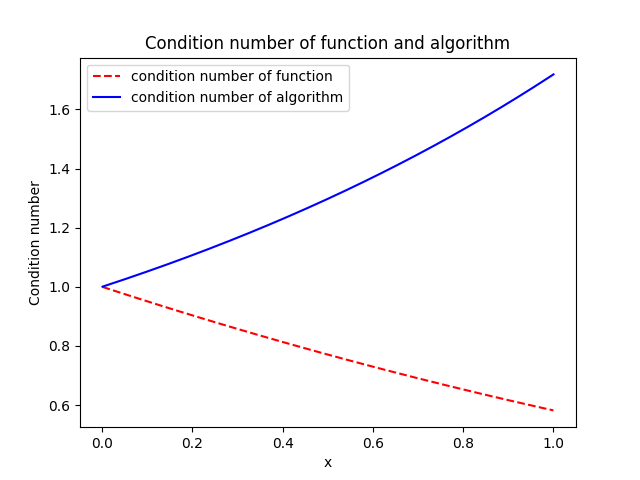
\includegraphics[width=0.5\textwidth]{../images/9_draw.png}
    \caption{The condition number of $f(x) = 1 - e^{-x}$ and the estimated condition number of an algorithm}
    \label{fig:9_draw}
\end{figure}

The figure shows that the condition number of both the function and the algorithm grows more distant from 1 as $x$ grows. So this question is more ill-conditioned as $x$ increases.

\section{Prove Lemma 4.68}

The lemma concentrates on the connection between the condition number and the singular values and the eigenvalues of a matrix. It follows
\begin{equation}
    \text{cond}_2 A = \frac{\sigma_{\text{max}}}{\sigma_\text{min}}.
    \label{eq:10_cond_A_singular}
\end{equation}

If $A$ is also normal, then we have 
\begin{equation}
    \text{cond}_2 A = \frac{|\lambda_{\text{max}}|}{|\lambda_{\text{min}}|}.
    \label{eq:10_cond_A_eigen}
\end{equation}

\subsection{Prove \cref{eq:10_cond_A_singular}}

With the definition 
\begin{align}
    \text{cond}_2 A &:= \|A\|_2 \|A^{-1}\|_2, 
    \label{eq:10_cond_A_def} \\
    \|A\|_2 &:= \sqrt{\lambda_{\max}(A^TA)}, 
    \label{eq:10_2norm_A_def} 
\end{align}

and the properties of SVD, we have 
\begin{equation}
    \begin{aligned}
        \sigma_{\max} &= \|A\|_2, \\
        \sigma_{\min} &= \|A^{-1}\|_2, \\
        \text{cond}_2 A &= \frac{\sigma_{\max}}{\sigma_{\min}}. \\
    \end{aligned}
    \label{eq:10_cond_A_singular_proof}
\end{equation}

\subsection{Prove \cref{eq:10_cond_A_eigen}}

When $A$ is normal, the eigenvalues of $A$ and $A^{T}$ are the same, so it follows
\begin{equation}
    \begin{aligned}
        \lambda_{\max}(A^T A) &= (\lambda_{\max}(A))^2 = \sigma_{\max}^2, \\
        \lambda_{\min}(A^T A) &= (\lambda_{\min}(A))^2 = \sigma_{\min}^2, \\
        \text{cond}_2 A &= \frac{\sigma_{\max}}{\sigma_{\min}} = \frac{|\lambda_{\max}|}{|\lambda_{\min}|}.
    \end{aligned}
    \label{eq:10_cond_A_eigen_proof}
\end{equation}

\section{Discuss the condition number of a root finding algorithm}

In this section, we consider a vector function $f: \mathbb{R} \to \mathbb{C}:$
\begin{equation}
    r = f(a_0, a_1, \cdots, a_{n - 1})
    \label{eq:11_r_def}
\end{equation}
for the problem of finding roots for the polynomial 
\begin{equation}
    q(x) = \sum_{i = 0}^n a_i x^i, \quad a_n = 1, a_0 \ne 0, a_i \in \mathbb{R}.
    \label{eq:11_polynomial_def}
\end{equation}

From the Lemma 4.63 in the textbook, we have the partial derivative of $f$ with respect to $a_i$ is
\begin{equation}
    \begin{aligned}
        \frac{\partial f}{\partial a_i}(a_0, a_1, \cdots, a_{n - 1}) &= \lim_{\varepsilon \to 0}\frac{f(x_0, x_1, \cdots, x_i + \varepsilon, \cdots, x_{n - 1}) - f(x_0, x_1, \cdots, x_i, \cdots, x_{n - 1})}{\varepsilon} \\
        &= \lim_{\varepsilon \to 0}\frac{r - \varepsilon \frac{r^i}{q'(r)} - r}{\varepsilon} \\
        &= -\frac{r^i}{q'(r)}.
    \end{aligned}
    \label{eq:11_partial_derivative}
\end{equation}

Denote $\alpha = (a_0, a_1, \cdots, a_{n - 1})$, then we have the component-wise condition number of $f$ based on the 1-norm as
\begin{equation}
    \begin{aligned}
        \text{cond}_f (\alpha) &= \sum_{i = 0}^{n - 1} \left|\frac{a_i \frac{r^i}{q'(r)}}{f(\alpha)}\right| \\
        &= \frac{1}{rq'(r)} \sum_{i = 0}^{n - 1} \left|a_i r^i\right|.
    \end{aligned}
    \label{eq:11_cond_f_1norm}
\end{equation}

For the Wilkinson example, we have $q(x) = \prod_{k = 1}^p (x - k) = \sum_{i = 0}^p a_i x^i$. The corresponding component-wise condition number is 
\begin{equation}
    \begin{aligned}
        \text{cond}_f (\alpha) &= \frac{1}{pq'(p)} \sum_{i = 0}^{p - 1} \left|a_i p^i\right| \\
        &= \frac{1}{p(p - 1)(p - 2)\cdots(p - p + 1)} (\prod_{i = 1}^p(1 + ip) - p^p) \\
        &= \frac{\prod_{i = 1}^p(1 + ip) - p^p}{p!},
    \end{aligned}
    \label{eq:11_cond_f_wilkinson}
\end{equation}
with the formula
\begin{equation}
    \begin{aligned}
        \sum_{i = 0}^{p - 1} |a_i p^i| &= \sum_{i = 0}^p |a_i p^i| - a_p p^p \\
        &= \sum_{i = 0}^p |a_i| p^i - p^p \\
        &= \sum_{i = 0}^p \sigma_i(1, 2, \cdots, p) p^i - p^p \\
        &= \prod_{i = 1}^p (1 + ip) - p^p
    \end{aligned}
    \label{eq:11_sum_formula}
\end{equation}
by using the generating function for the elementary symmetric polynomials of Definition 3.42 in the textbook.

For $p = 20, 30, 40$, the component-wise condition number of $f$ are $1.3 \times 10^{26}, 2.4 \times 10^{44}, 1.3 \times 10^{64}$, respectively. The result is corresponding to that in the Wilkinson example, which implies the problem of root finding for polynomials with very high degrees is hopeless.

\section{Change the precision of division and give an example conflicting with the conclusion}

In this task, we suppose the division of two FPNs is calculated in a register of precision $2p$ instead of at least $2p + 1$.

For the binary FPN, we have $\epsilon_M = 2^{1 - p}, \epsilon_u = 2^{-p}$. Assuming $p = 3, a = (1.00)_2, b = (1.11)_2$, then 
\begin{equation}
    M_a = (1.00)_2 \times 2^0, M_b = (1.11)_2 \times 2^0, M_a / M_b = (0.100100\cdots)_2, e_c = e_a - e_b = 0,
    \label{eq:12_division_binary}
\end{equation} 
which implies $M_c = (1.0010)_2 \times 2^{-1}$, and by rounding it to precision $p$ it becomes 
\begin{equation}
    c = (1.00)_2 \times 2^{-1}.
    \label{eq:12_division_binary_result}
\end{equation}

So with $\text{fl}(\frac{a}{b}) = \frac{a}{b}(1 + \delta)$, we can get $\delta = c \frac{b}{a} - 1 = -\frac{1}{8}$, and its absolute value equals to $\epsilon_u$, which leads to contradiction.

\section{Discuss the range of absolute accuracy}

If we start the bisection method with the interval $[128,\ 129]$, with the theorem 
\begin{equation}
    \forall a, b \in \mathcal{F},\ a \odot b \in \mathcal{R(F)} \Rightarrow \text{fl}(a \odot b) = (a \odot b)(1 + \delta),\ |\delta| < \epsilon_u,
    \label{eq:13_bisection_theorem}
\end{equation}
we can get the upper bound of the absolute accuracy as $(a \odot b)\delta$, and it can be approximated by $2^7 \times 2^{-24} = 2^{-17} \approx 7.63 \times 10^{-6} > 10^{-6}$, so we can't compute the root with absolute accuracy $< 10^{-6}$.

\section{Explain the inaccuracy of cubic splines in some cases}

From the Theorem 3.7 in the textbook, we have the linear system of complete cubic splines as follows.
\begin{equation}
    \begin{bmatrix}
        2 & \mu_2 & & & & & \\
        \lambda_3 & 2 & \mu_3 & & & & \\
        & & \ddots & & & & \\
        & & \lambda_i & 2 & \mu_i & & \\
        & & & & \ddots & & \\
        & & & & \lambda_N & 2 & \mu_{N - 2} \\
        & & & & & \lambda_{N - 1} & 2
    \end{bmatrix}
    \mathbf{m} = \mathbf{b},
    \label{eq:14_cubic_spline_system}
\end{equation}
where 
\begin{equation}
    \mu_i = \frac{x_i - x_{i - 1}}{x_{i + 1} - x_{i - 1}},\quad \lambda_i = \frac{x_{i + 1} - x_i}{x_{i + 1} - x_{i - 1}}.
    \label{eq:14_cubic_spline_coefficients}
\end{equation}

If the distance between every two adjacent points is the same, we have $\mu_i = \lambda_i = \frac{1}{2},\ \forall i = 1, 2, \cdots, N$.

With \cref{eq:10_cond_A_singular}, we can know that the condition number is close to 1 when the element of matrix is close. Consequently, the condition number is large when the distance between two adjacent points is much smaller than those of other adjacent pairs, which makes the matrix ill-conditioned.

\section{Exercise 4.33: Addition of two FPNs}

In this exercise, we consider the calculation of $c := \text{fl}(a + b)$ with $a = 1.234 \times 10^4$ and three values of $b$.

\subsection{$b = 8.769 \times 10^4$}

\begin{enumerate}
    \item $e_c \leftarrow 4$.
    \item $m_c \leftarrow 10.003$.
    \item $m_c \leftarrow 1.0003;\ e_c \leftarrow 5$.
    \item do nothing.
    \item $m_c \leftarrow 1.000$.
    \item $c = 1.000 \times 10^5$.
\end{enumerate}

\subsection{$b = -5.678 \times 10^0$}

\begin{enumerate}
    \item $b \leftarrow -0.0005678 \times 10^4;\ e_c \leftarrow 4$.
    \item $m_c \leftarrow 1.2334322$.
    \item do nothing.
    \item do nothing.
    \item $m_c \leftarrow 1.233$.
    \item $c \leftarrow 1.233 \times 10^4$.
\end{enumerate}

\subsection{$b = -5.678 \times 10^3$}

\begin{enumerate}
    \item $b \leftarrow -0.5678 \times 10^4;\ e_c \leftarrow 4$.
    \item $m_c \leftarrow 0.6662$.
    \item $m_c \leftarrow 6.662;\ e_c \leftarrow 3$.
    \item do nothing.
    \item do nothing.
    \item $c \leftarrow 6.662 \times 10^3$.
\end{enumerate}

\section{Exercise 4.42: Give an example of the minimal rounding error}

By sorting the positive number $a_i > 0$ according to their magnitudes and carry out the addition in this ascending order, we can decrease the influence of rounding error.

Here is a segment of code in Python to implement this idea:
\begin{lstlisting}[language = python]
    result1 = 0
    result2 = 0
    
    num = [1, 1e-9, 9e-10, 8e-10, 7e-10, 6e-10, 5e-10, 4e-10, 3e-10, 2e-10, 1e-10]
    
    for i in range(0, len(num)):
        result1 += num[i]
        result2 += num[len(num)-1-i]
    
    print(result1)
    print(result2)   
\end{lstlisting}

and the output is 
\begin{lstlisting}
    1.0000000055000005
    1.0000000055
\end{lstlisting}

We can see that by sorting the numbers in ascending order, the rounding error is decreased, as the real result equals to 1.0000000055.

\section{Exercise 4.43: Derive a sum and compare it with another result}

For $\text{fl}(a_1b_1 + a_2b_2 + a_3b_3)$, we have
\begin{equation}
    \begin{aligned}
        \text{fl}(a_1b_1 + a_2b_2 + a_3b_3) &= \text{fl}(\text{fl}(\text{fl}(a_1b_1) + \text{fl}(a_2b_2))+\text{fl}(a_3b_3)) \\
        &= ((a_1b_1(1 + \delta_1) + a_2b_2(1 + \delta_2))(1 + \delta_3) + a_3b_3(1 + \delta_4))(1 + \delta_5),
    \end{aligned}
    \label{eq:15_fl_sum}
\end{equation}
where $|\delta_i| < \epsilon_u$ for $i = 1, 2, 3, 4, 5$.

For $\text{fl}(\sum_i \prod_j a_{i, j})$, it follows
\begin{equation}
    \text{fl}(\sum_i \prod_j a_{i, j}) = \text{fl} \sum_i \text{fl}(\prod_j a_{i, j}) = (1 + \delta)\sum_{i = 1}^m (1 + \delta_i) \prod_{j = 1}^n a_{i, j}(1 + \delta_{i, j}).
    \label{eq:15_fl_prod_sum} 
\end{equation}

The results show that the order of multiplication does not influence the rounding error, while the order of addition does.

\section{Exercise 4.80: Change the form of a function and get a better result}

In this section, we consider the function 
\begin{equation}
    f(x) = \frac{1 - \cos x}{\sin x} = \frac{\sin x}{1 + \cos x}.
    \label{eq:16_f}
\end{equation}

It is easy to compute that 
\begin{equation}
    \text{cond}_f (x) = \frac{x}{\sin x}.
    \label{eq:16_cond_f}
\end{equation}

With the formula $f(x) = \frac{\sin x}{1 + \cos x}$, we have 
\begin{equation}
    f_A(x) = \frac{\sin x(1 + \delta_1)}{(1 + \cos x(1 + \delta_2))(1 + \delta_3)}(1 + \delta_4),
    \label{eq:16_fA}
\end{equation}
where $|\delta_i| < \epsilon_u$ for $i = 1, 2, 3, 4$. Neglecting the quadratic terms of $O(\delta_i^2)$, the above equivalent to
\begin{equation}
    f_A(x) = \frac{\sin x}{1 + \cos x}(1 + \delta_1 + \delta_4 - \delta_3 - \delta_2 \frac{1 + \cos x}{\cos x}),
    \label{eq:16_fA_simplified}
\end{equation}
hence we have $\varphi(x) = 3 + \frac{1 + \cos x}{\cos x}$ and 
\begin{equation}
    \text{cond}_A (x) \leqslant \frac{\sin x}{x} \left(3 + \frac{1 + \cos x}{\cos x}\right).
    \label{eq:16_cond_A}
\end{equation}

Consequently, $\text{cond}_A(x)$ may be unbounded as $x \to \frac{\pi}{2}$. On the other hand, $\text{cond}_A (x)$ is controlled by 5 as $x \to 0$. 

\section*{ \center{\normalsize {Acknowledgement}} }

In the process of writing this report, I use \href{https://kimi.moonshot.cn/}{\textit{Kimi AI}} to help me translate something and write this report by \TeX.

\end{document}